% Created 2023-10-31 di 19:57
% Intended LaTeX compiler: pdflatex
\documentclass[bigger]{beamer}
\usepackage[utf8]{inputenc}
\usepackage[T1]{fontenc}
\usepackage{graphicx}
\usepackage{longtable}
\usepackage{wrapfig}
\usepackage{rotating}
\usepackage[normalem]{ulem}
\usepackage{amsmath}
\usepackage{amssymb}
\usepackage{capt-of}
\usepackage{hyperref}
\usepackage{graphicx}
\usetheme{default}
\author{Jeroen van Riel}
\date{November 2023}
\title{Learning to Control Traffic}
\hypersetup{
 pdfauthor={Jeroen van Riel},
 pdftitle={Learning to Control Traffic},
 pdfkeywords={},
 pdfsubject={},
 pdfcreator={Emacs 28.1 (Org mode 9.7)}, 
 pdflang={English}}
\usepackage{natbib}
\begin{document}

\maketitle

\begin{frame}[label={sec:org0e15610}]{Learning problem}
\begin{itemize}
\item set of problem instances \(\mathcal{I}\)
\item distribution \(P\) over instances
\item set of algorithms \(\mathcal{A}\)
\item measure of optimality \(m : \mathcal{I} \times \mathcal{A} \rightarrow \mathbb{R}\)
\end{itemize}

\vfill
based on \citep{bengioMachineLearningCombinatorial2020} 
\end{frame}
\begin{frame}[label={sec:org46a2ad2}]{Learning problem}
\begin{itemize}
\item general learning objective
\end{itemize}
\begin{align}
\min_{a \in \mathcal{A}} \mathbb{E}_{i \sim P} \; m(i, a)
\end{align}

\begin{itemize}
\item no access to \(\mathcal{I}\) or \(P\), so use samples
\end{itemize}
\begin{align}
\min_{a \in \mathcal{A}} \sum_{i \in D_{\mathit{train}}} \frac{1}{|D_\mathit{train}|} m(i, a)
\end{align}
\end{frame}

\begin{frame}[label={sec:orgefe7fb3}]{Learning problem}
\begin{itemize}
\item demonstration
\item experience
\end{itemize}
\end{frame}


\begin{frame}[label={sec:orge4c6b7c}]{Demonstration}
\begin{itemize}
\item parameterization of algorithms, e.g., by using neural network with weights \(\theta \in \mathbb{R}^p\)
\end{itemize}
\begin{align}
\min_{\theta \in R^p} \mathbb{E}_{i \sim P} m(i, a(\theta))
\end{align}
\end{frame}

\begin{frame}[label={sec:org72eda48}]{Experience}
\begin{itemize}
\item greedy TSP heuristic = picking next node
\end{itemize}
\end{frame}

\begin{frame}[label={sec:orgf0b6253}]{Learning to cut (example)}
\end{frame}


\begin{frame}[label={sec:orge8a68b8}]{Job shop}
\begin{itemize}
\item \(m\) machines
\item \(n\) jobs
\item fixed machine order for each job
\end{itemize}
\end{frame}

\begin{frame}[label={sec:orgbe6a583}]{Disjunctive graph}
\begin{itemize}
\item directed graph \(G=(N, \mathcal{C}, \mathcal{D})\)
\item conjunctive arcs
\item disjunctive arcs
\end{itemize}

\begin{figure}
  \centering
  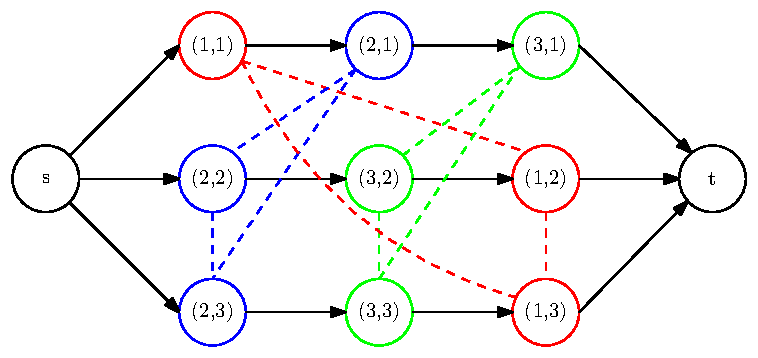
\includegraphics[width=0.9\textwidth]{disjunctive-graph.pdf}
\end{figure}
\end{frame}

\begin{frame}[label={sec:org51ef9ba}]{Job shop MILP}
\begin{itemize}
\item makespan objective
\item mixed-integer linear program
\end{itemize}

\scalebox{0.85}{\parbox{.9\linewidth}{
\begin{align*}
\text{minimize } & C_{\text{max}} \\
y_{ij} + p_{ij} &\leq y_{kj}  & \text{ for all } (i,j) \xrightarrow{} (k,j) \in \mathcal{C} \\
y_{il} + p_{il} &\leq  y_{ij} \text{ or } y_{ij} + p_{ij} \leq y_{il}  & \text{ for all } (i,l) \text{ and } (i,j), i =1, \dots,m \\
y_{ij} + p_{ij} &\leq C_{\text{max}} & \text{ for all } (i,j) \in N \\
y_{ij} &\geq 0 & \text{ for all } (i,j) \in N
\end{align*}
}}
\end{frame}

\begin{frame}[label={sec:org61b622c}]{Traffic scheduling problem}
\begin{itemize}
\item total completion time
\item release dates
\item chains
\item setup times (switch-over)
\end{itemize}
\end{frame}

\begin{frame}[label={sec:orgd630654}]{References}
\begingroup
\renewcommand{\section}[2]{}
\bibliography{references}
\bibliographystyle{plainnat}
\endgroup

\(\;\)
\end{frame}
\end{document}